% chapter 7
\chapter{Physical Design}
\label{chap:07_physical_design}

%\begin{figure}[!htbp]
\section{Scripts}
\label{sec:phy_scripts}

The completion of this project entails converting the synthesized netlists into a physical layout for the DLX processor, using Cadence Innovus as discussed in Section~\ref{sec:software}. \\

As with the simulation and synthesis phases, a script named \textbf{runphy.sh} was developed (see Appendix~\ref{app:runphy}). This script initializes the working environment and automatically retrieves the updated files for placement and routing from the folders designated for architecture synthesis. \\

To execute the script, navigate to the appropriate directory, specifically \texttt{dlx/phy}, and run the following command:
\begin{lstlisting}[style=MyShell]
 > ./runphy.sh
\end{lstlisting}

Note that this script does not automatically initiate the design-generating software. To launch Innovus, you must manually enter the following command in the terminal:
\begin{lstlisting}[style=MyShell]
 > innovus
\end{lstlisting}

Within Innovus, a significant portion of the design process was automated using logs generated by the software. By executing three simple commands, one can complete the design generation.

The first command runs the \texttt{dlx.globals} script (see Appendix~\ref{app:runphy}) that was provided as part of the course materials to import the design:
\begin{lstlisting}[style=MyShell]
 > source dlx.globals
\end{lstlisting}

The second command executes the \texttt{phy.tcl} script (see Appendix~\ref{app:phy}) to generate the actual physical design:
\begin{lstlisting}[style=MyShell]
 > source phy.tcl
\end{lstlisting}

Lastly, the command \texttt{analyses.tcl} (see Appendix~\ref{app:analyses}) is used to generate the required reports:
\begin{lstlisting}[style=MyShell]
 > source analyses.tcl
\end{lstlisting}

\section{Workflow}
The overall procedure was conducted in alignment with the guidelines and protocols established in the corresponding laboratory session. The comprehensive workflow included several critical steps, each essential for successful physical design implementation. These phases are detailed as follows:

\begin{itemize}
	\item \textbf{Design importation}: this is the initial phase where Innovus is configured to locate the paths to the libraries essential for the design. The synthesized description of the circuit is read, and a configuration file is imported, setting the correct references to the libraries. The design is then fully imported, complete with the correct cell references and the RTL Verilog description.
	
	\item \textbf{Floorplan construction}: in this stage, Innovus establishes the area that will be designated for the cells, as well as the space for power supply routing. Parameters like Core aspect ratio and Utilization are specified, and the core margins are defined. This lays the groundwork for how cells will be placed in the layout.
	
	\item \textbf{Power network planning and routing}: this phase involves creating power and ground rings around the core boundary using high metal layers to minimize congestion. The channel defined will be filled with two metal rings for power and ground, respectively. Additional vertical stripes are added to better distribute power across the chip.
	
	\item \textbf{Cell arrangement}: during this phase, all the standard cells are systematically placed within the predefined rows of the floorplan. Care is taken to place the cells away from power and ground stripes to avoid congestion issues.
	
	\item \textbf{Signal trace routing}: here, the logical connections between the cell pins are turned into actual metal traces. This stage involves defining the routes for signal propagation throughout the chip. Various metal layers are employed to ensure efficient connections while minimizing the likelihood of issues such as signal interference or routing congestion.
	
	\item \textbf{Timing analysis and design evaluation}: the final phase focuses on optimizing the design to meet timing constraints. After the routing is done, Clock-Tree-Synthesis (CTS) and Post-CTS optimizations can be performed to make sure that the design meets the specified timing requirements.
\end{itemize}

Each of these steps contributes to the successful realization of the chip's physical design, ensuring not only its functional capabilities but also its operational efficiency.

\section{Results}
The culmination of the physical design process is captured in a comprehensive post-routing schematic. A detailed graphical representation of this final layout is presented in Figure~\ref{fig:physical_dlx}. \\

\begin{figure}[!htbp]
    \centering
    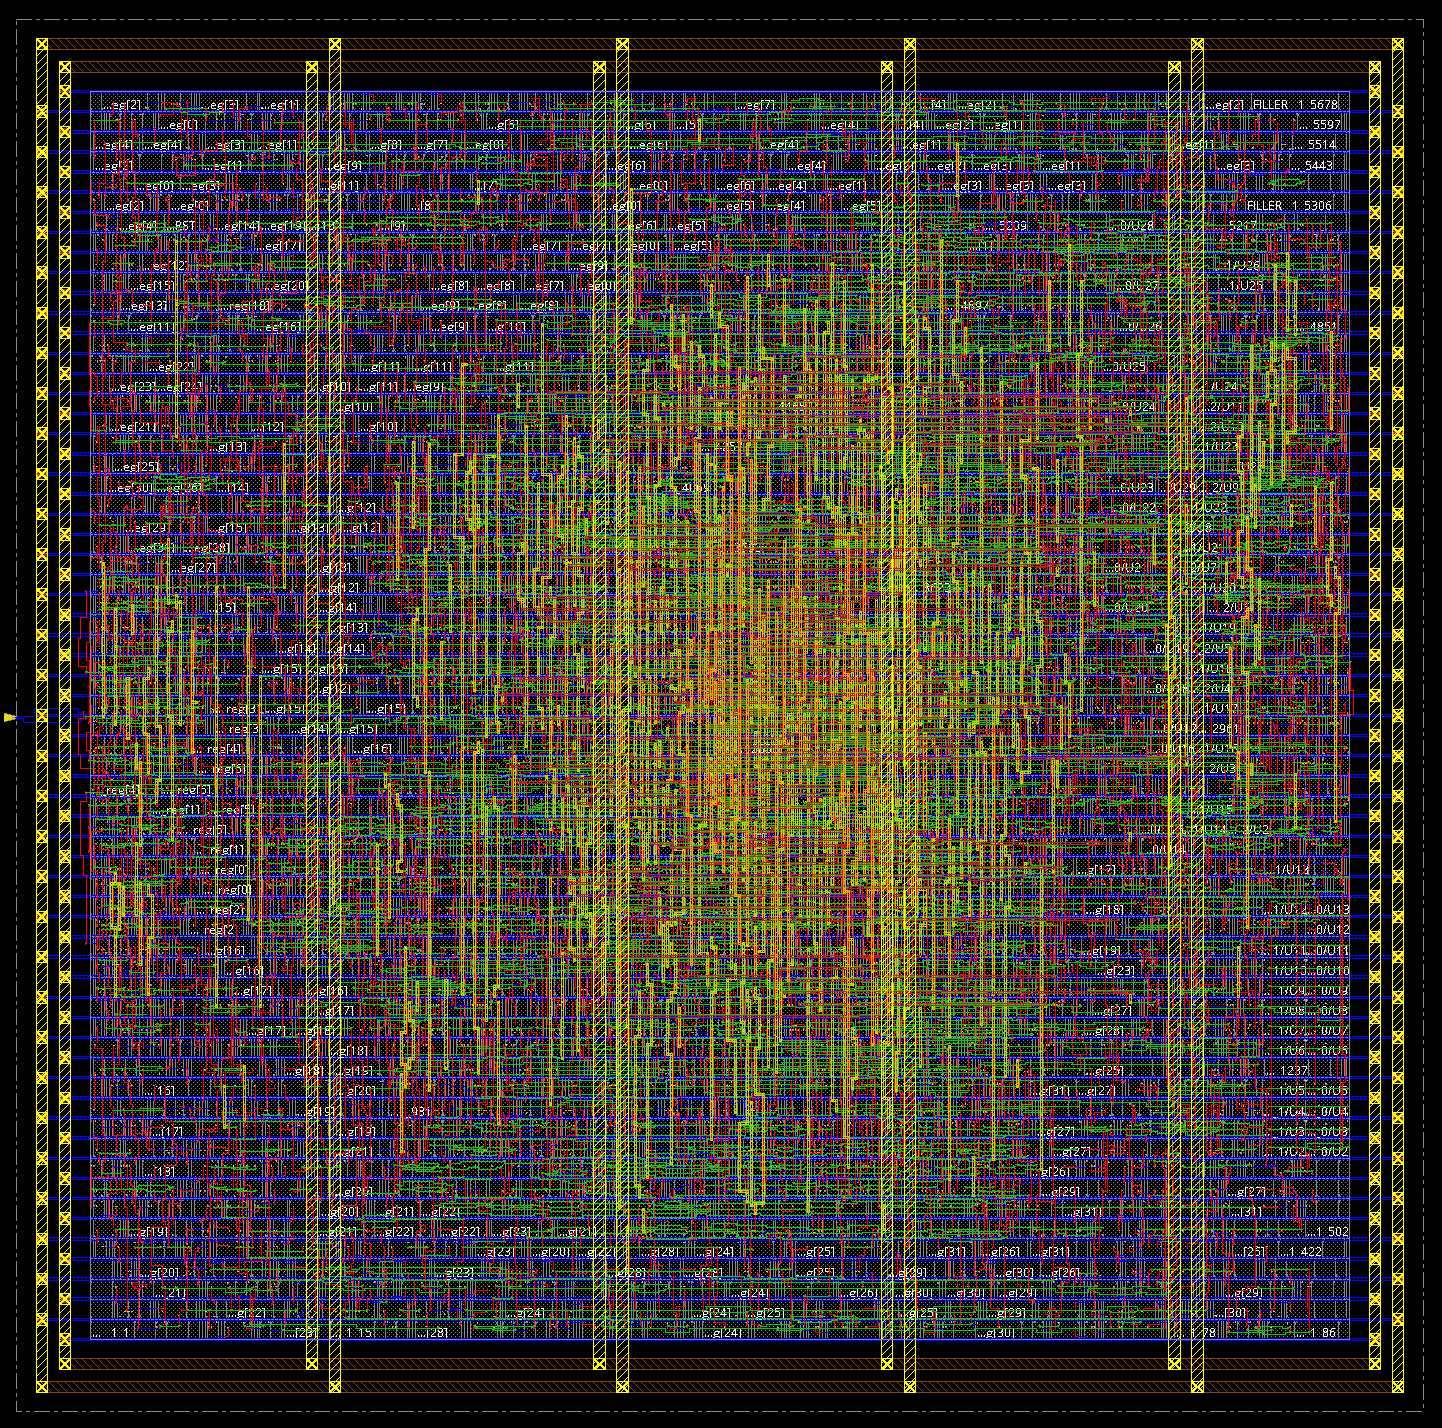
\includegraphics[width=0.9\textwidth]{source/figures/physical_dlx.png}
    \caption{Finalized schematic illustrating the placement and routing outcome}
    \label{fig:physical_dlx}
\end{figure}

\paragraph{Area}
Complementing the schematic representation, a set of quantitative metrics has also been assembled to provide additional layers of evaluation. These metrics offer a numerical perspective on the design's complexities and efficiencies. The salient details concerning the gate count, the number of cells utilized, and the total area occupied by each hierarchical level of modules in the design are summarized in Table~\ref{tab:phy_results}. \\

\begin{table}[!htbp]
	\centering
	\begin{tabular}{clccc}
		\toprule
		Level & Module & Gates & Cells & Area [$\mu m^2$] \\
		\midrule
		0 & DLX & 16992 & 9127 & 13560.1 \\
		1 & CU & 276 & 165 & 220.8 \\
		1 & DATAPATH & 16708 & 8959 & 13333.5 \\
		2 & DATAPATH/RF & 6337 & 2755 & 5056.9 \\
		2 & DATAPATH/ALU & 4841 & 3592 & 3863.4 \\
		3 & DATAPATH/ALU/MUL & 1792 & 1244 & 1430.3 \\
		3 & DATAPATH/ALU/SUM & 772 & 566 & 616.1 \\
		\bottomrule
	\end{tabular}
	\caption{Detailed summary of gate counts and area measurements}
	\label{tab:phy_results}
\end{table}

This analysis offers valuable insights into the distribution of gates, cells and area across the hierarchical design modules. With an overall gate count of 16992 and an aggregated physical design area of 13560.1 $\mu m^2$, the architecture exhibits a relatively small hardware footprint. The Datapath module accounts for almost the entire area, constituting approximately 98\% of the overall gate count and physical area. Within this module, the Register File and Arithmetic Logic Unit (ALU) are the dominant sub-modules, occupying 5056.9 $\mu m^2$ and 3863.4 $\mu m^2$ of area respectively. \\

Upon further examination of the ALU, it is noteworthy that the Multiplier (MUL) sub-module alone occupies around 1430.3 $\mu m^2$, highlighting the complexity associated with implementing multiplication operations. The ALU's P4 Adder (SUM) sub-module also proves to be a significant component of the ALU, ranking second in terms of area with 3863.4 $\mu m^2$. \\

The Control Unit (CU) is exceptionally compact, featuring only 276 gates and 220.8 $\mu m^2$ of area. This underscores the efficiency of the control logic in the DLX architecture. \\

Interestingly, the average gate area is calculated to be 0.7980 $\mu m^2$, serving as a benchmark for evaluating the granularity of the design.

\paragraph{Timing}
The Tables~\ref{tab:optdesign_postroute_summary} and~\ref{tab:optdesign_postcts_summary} provide a comprehensive evaluation of the setup and hold times for various routing modes, both pre- and post-optimization. Prior to optimization, the Worst Negative Slack (WNS) in the setup mode for \textbf{all} paths is marginally better than the \textbf{default} mode at 0.014~$ns$ and also the \textbf{reg2reg} mode shows a slightly higher value of 0.090~$ns$. No timing violations were reported. After Clock Tree Synthesis (CTS), the setup time improved slightly in the \textbf{all} and \textbf{default} modes to 0.008~$ns$. \\

In the hold mode, a single violating path was observed pre-optimization for the \textbf{all} and \textbf{default} modes, indicating a minor issue with data stability. This was resolved post-optimization as evidenced by the absence of violating paths and a WNS of 0.000~$ns$. The \textbf{reg2reg} mode was robust in both scenarios, demonstrating no hold time violations. \\

\begin{table}[!htbp]
    \centering
    \begin{minipage}{0.48\textwidth}
        \centering
        \begin{tabular}{lccc}
            \toprule
            \textbf{Setup Mode} & all & reg2reg & default \\
            \midrule
            WNS [$ns$]: & 0.014 & 0.090 & 0.014 \\
            TNS [$ns$]: & 0.000 & 0.000 & 0.000 \\
            Violating Paths: & 0 & 0 & 0 \\
            All Paths: & 224 & 54 & 217 \\
            \midrule
            \textbf{Hold Mode} & all & reg2reg & default \\
            \midrule
            WNS [$ns$]: & -0.001 & 0.008 & -0.001 \\
            TNS [$ns$]: & -0.001 & 0.000 & -0.001 \\
            Violating Paths: & 1 & 0 & 1 \\
            All Paths: & 224 & 54 & 217 \\
            \bottomrule
        \end{tabular}
        \caption{optDesign postRoute summary}
        \label{tab:optdesign_postroute_summary}
    \end{minipage}
    \hfill
    \begin{minipage}{0.48\textwidth}
        \centering
        \begin{tabular}{lccc}
            \toprule
            \textbf{Setup Mode} & all & reg2reg & default \\
            \midrule
            WNS [$ns$]: & 0.008 & 0.087 & 0.008 \\
            TNS [$ns$]: & 0.000 & 0.000 & 0.000 \\
            Violating Paths: & 0 & 0 & 0 \\
            All Paths: & 224 & 54 & 217 \\
            \midrule
            \textbf{Hold Mode} & all & reg2reg & default \\
            \midrule
            WNS [$ns$]: & 0.000 & 0.009 & 0.000 \\
            TNS [$ns$]: & 0.000 & 0.000 & 0.000 \\
            Violating Paths: & 0 & 0 & 0 \\
            All Paths: & 224 & 54 & 217 \\
            \bottomrule
        \end{tabular}
        \caption{optDesign postCTS summary}
        \label{tab:optdesign_postcts_summary}
    \end{minipage}
\end{table}

These observations underscore the efficacy of the optimization strategies implemented, especially in resolving the minor hold time violation while maintaining excellent setup times.
